\section{Pitfalls}

Schlussendlich wollen wir noch Situationen aufzeigen, an denen der Algorithmus scheitert.
Die erste Möglichkeit dafür besteht darin, dass die Quadratur zu ungenau ist, und somit die \enquote{korrekten} Singulärwerte nicht mehr von den zusätzlichen Werten zu unterscheiden sind.
In Abbildung \ref{fig:plot4} sieht man, wie sich die approximierten Singulärwerte bei unterschiedlicher Anzahl von Quadraturknoten verhalten.
Ab $\texttt{m} \geq 20$ Quadraturknoten aufwärts ist bereits ein Sprung zwischen den echten und zusätzlichen Werten zu erkennen, der sich bei steigender Anzahl noch verdeutlicht.

\begin{figure}[H]
  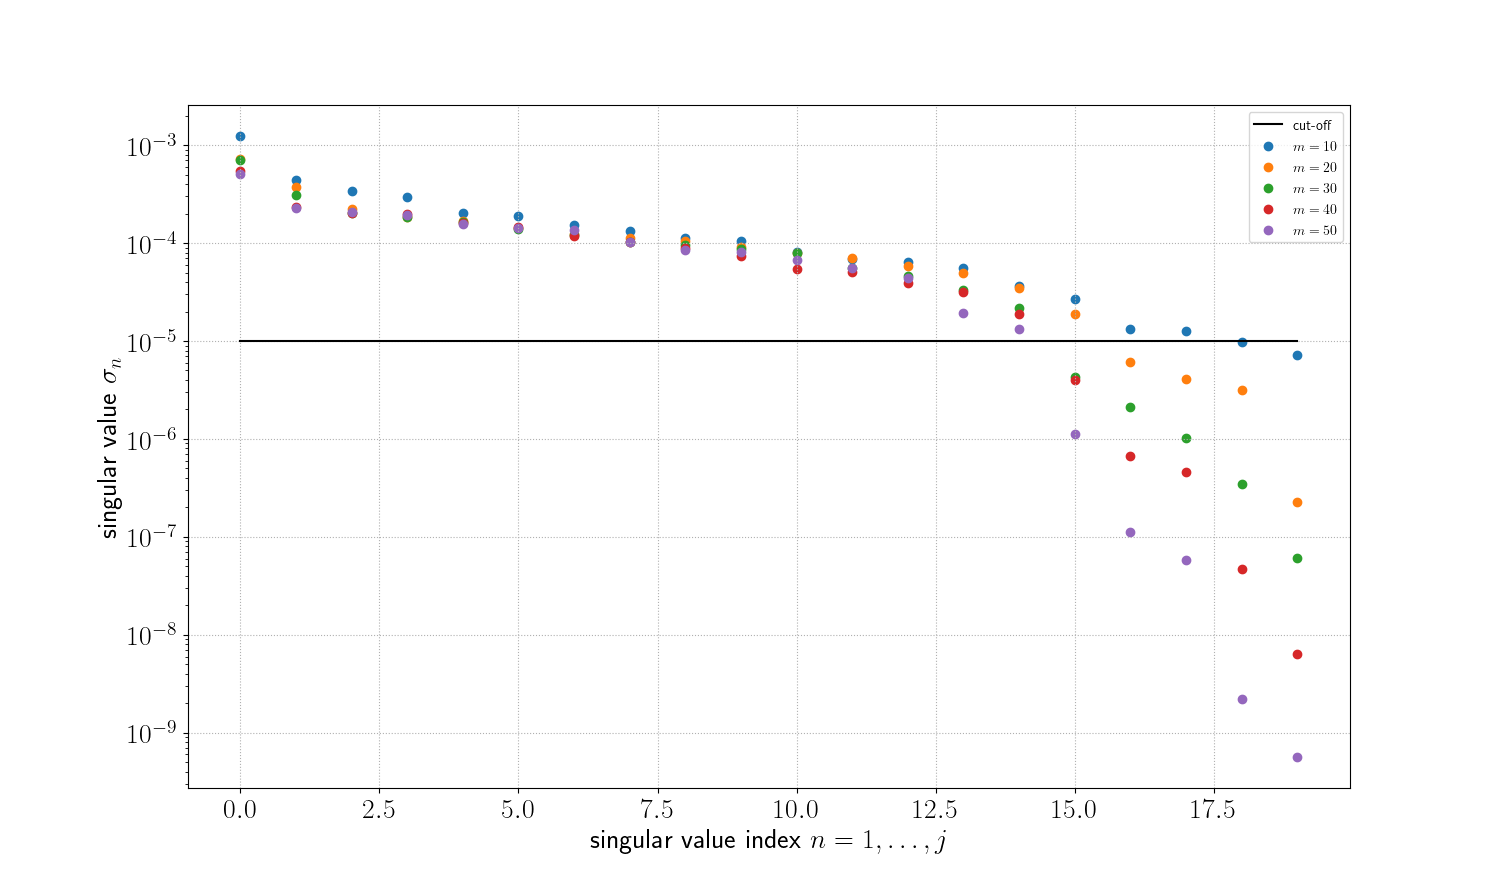
\includegraphics[width = \linewidth]{Plots/singulaerwerte_quadraturknoten.png}
  \caption{Singulärwerte in Abhängigkeit von der Anzahl der Quadraturknoten}
  \label{fig:plot4}
\end{figure}

Das zweite Hauptproblem ist, wenn die Zufallsmatrix zu klein gewählt wird.
Sollte die Zufallsmatrix weniger Spalten haben, als wir Eigenwerte innerhalb unserer Kurve erwarten, könnte man ja noch hoffen, zumindest einen Teil der Eigenwerte korrekt approximieren zu können.
Wie man in Abbildung \ref{fig:plot5} sieht, können wir in der Regel nicht einmal das erwarten.

\begin{figure}[H]
  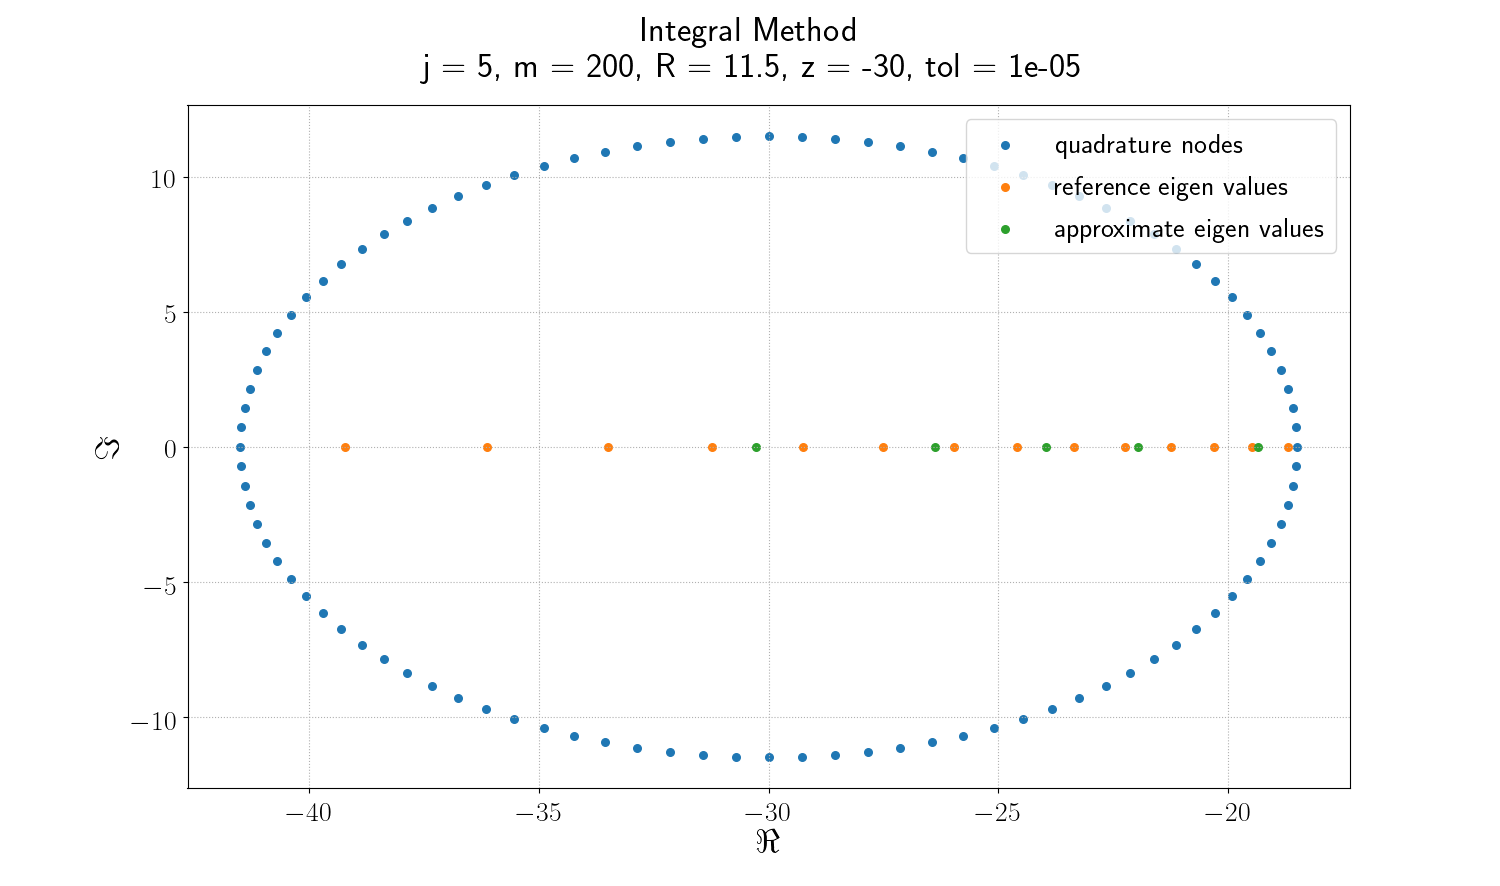
\includegraphics[width = \linewidth]{Plots/zufallsmatrix_zu_klein.png}
  \caption{Zu kleine Zufallsmatrix}
  \label{fig:plot5}
\end{figure}
